% 补充:是否加入tenure? 能否很好地解释tenure 和 age的区别?



\documentclass{article}
\usepackage[utf8]{inputenc}
\usepackage[english]{babel}
\usepackage[]{amsthm} %lets us use \begin{proof}
\usepackage[]{amssymb} %gives us the character \varnothing
\usepackage{amsmath}
\usepackage[shortlabels]{enumitem}
\usepackage{CJKutf8}
\usepackage{array,multirow}

\usepackage{booktabs}
\usepackage{dcolumn}
\usepackage{float}
\usepackage{graphicx}


\title{Incentivizing Lockdown Policies: \\An Agency Theory Explanation}
\author{Qitian Hu 18340686048}
%\end{CJK}
%This information doesn't actually show up on your document unless you use the maketitle command below

\linespread{1.3}
\usepackage[margin=1.2in]{geometry}
\usepackage{graphicx}


\begin{document}
\begin{CJK}{UTF8}{gbsn}
\maketitle %This command prints the title based on information entered above
\begin{abstract}
	In this paper, I connect the literature on incomplete contract and principal-agent problem to the policy choices of local Chinese officials during the COVID-19 pandemic. With evidence from multiple datasets, I demonstrate that the younger the city secretary is, the riskier she is. This phenomenon might be connected with by the intentional bias in policy advertisements.
\end{abstract}


\section{Introduction}
Ever since December 2019, the novel COVID-19 virus has rapidly spread around world. As the country in which the virus is first identified, Chinese government has adopted a number of policy measures to suppress the virus, including enforcing strict quarantines, prohibiting gatherings, and locking down entire cities. Pattern of these policy measures is not entirely determined the by spread of virus or socio-economic conditions of the city. For example, while Inner Mongolia is a large, sparsely populated region, it adopts strict quarantine policies \cite{inner mongolia}, and Dongyin in Shangdong province, a city without any confirmed case, locked itself down as early as the end of January \cite{yuhang}. These instances show that the policy choice is not entirely a rational choice to balance virus control and socio-economic life, and must have involved the personal calculations of the city-level officials. 


\subsection{Chinese politics and COVID-19} 

The internal mechanism of Chinese government would be depicted from the incomplete contract and ownership perspective. Due to the limit of any predetermined allocations, the owner of capital usually have the residual right of control, and the ownership structure has crucial influence on the incentive structure \cite{holmstrom and roberts 1998}. Chinese government operates in a similar central-local governance structure. The upper-level government chooses delegates to lead local governments, and uses a different set of control rights to solve the incomplete contract between them. Based on the administrative subcontracting theory of Chinese governmance, there are three of such control rights that are particularly important \cite{zxg} : 

\begin{enumerate}
  \item The right to set goals. e.g. the Chinese Central government urges local governments to tackle COVID-19.
  \item The right of inspection. e.g. provincial or central governments examines whether the quarantine measures are taken. 
  \item The right of allocation (reward and punishment). e.g. central or provincial governments punish officials that failed to contain COVID-19 \cite{chezhi}.
\end{enumerate}

If upper-level governments have perfect control to these goals, they can effectively make the lower-level governments. 
However, facing the unique and urgent COVID-19 crisis, upper-level governments are not able to perfectly use these rights to tackle the virus. The most important friction is that the long-lasting incentive for economic development will complicate the goal of containing COVID-19. In China, upper-level governments select officials based on the objective economic performance of the corresponding region, and uses ranking to allocate the limited promotion opportunities. This "GDP Championship" creates a deep-rooted investment and production-driven policy pattern, and it has created significant difficulty when the central government tried to set up new goals like environment protection \cite{gdp contest}. 

In the early weeks of the pandemic, its infectivity and lethality are still unknown, thus local leaders face the decision that whether to adopt strict quarantine policy at the cost of economic development, or to take a bet that the virus will not attack her region and allow more socio-economic activities. I focus my analysis on the city level, because based on data I collect, it is the smallest administrative unit that has sufficient autonomy on COVID policies. I also argue that the policy decisions of individual cities is primarily made by party secretary of the city. The reason is that while mayors are responsible to the day-to-day operations, the party secretary has the final say. During the pandemic, Chinese cities form "Leading Groups" (疫情防控领导小组) to coordinates different bureaus and institutions; party secretary is almost always the leader of that group.

Decision of the party secretary is affected by numerous factors, but I will focus on age. The forced age of retirement is 60 for city-level leaders \cite{tuixiu}. If they have not been promoted by then, they will 'retire' to unimportant positions. Evidence show that this rule has strong incentive implications on policies on environmental protection and city construction \cite{mayor age effect, mayor age effect2}. 

As a summary, I argue that the lockdown policy choice in the early weeks in Chinese cities can be approximated by a principal-agent setting, where the party secretary (agent) faces two policy choices: no lockdown (risky, but has economic benefits) or enforce lockdown (safer, at the cost of economic development). In particular, I am interested in the ways age and career concerns affects risk preference.

%
%\begin{enumerate}
%  \item Chinese government 行政发包制-Administrative Subcontracting
%  \item incentivizing local officials: age, promotion, GDP contest 
%  \item 官员的年龄
%  \item covid management system : 指挥部 
%  \item how to understand COVID 19 in this contest -- risk
%\end{enumerate}

%\paragraph{formalize this incentive structure}
%How to understand this incentive system: 
%\begin{enumerate}
%  \item general, most important incentive is economic development
%  \item but COVID is a huge RISK, failing this can result in dismissal
%\end{enumerate}
%
%* General 
%* risk aversion 
%* effort input: young willing to make more effort 

\subsection{Literature on principal-agent problem} 

The setting above is similar to a number of classical models in corporate governance, where the principal are the shareholders and agent the manager. Similar to party secretaries, managers also concern their careers and adjust the risk and benefit of their investment choices accordingly. However, prior theoretical works offer conflicting prediction on this topic, and I will examine representative works in each strand.

%\begin{enumerate} 
%  \item principal and agent face different reward function -- prisoner's dilemma  最好别的城市都lockdown, 就自己放松 
%  \item principal want total control, but agent want to maximize it's performance 
%  \item risk and career prospect: 
%\end{enumerate}



\subsubsection{younger managers are risk-averse}
The first strand of literature argues that in a principal-agent setting, younger managers should be more sensitive to risk, mainly due to their career concerns. Two important models, addressing reputation gaining from two different perspectives, is illustrated here.

In his 1999 paper\cite{holmstrom1999}, Holmstrom developed a model to characterize the effort distribution of a manager in a dynamic setting with career concerns. The performance of a manager at time $t$ is determined by 
$$
y_{t}=\eta+a_{t}+\varepsilon_{t}, \quad t=1,2, \ldots, y^{t-1} = \{y_i\}_{i=0}^{t-1}
$$
where $\eta$ is the manager's ability, $a_{t} \in[0, \infty]$ her labor input and $\varepsilon_{t}$ is a stochastic noise term. The principal pays according to the expected value of $\eta$ and effort level, based on the information set available at time $t$, $y^{t-1}$. 

Thus the wage at $t$ is given by:
$$
w_{t}=E\left[y_{t} \mid y^{t-1}\right]=E\left[\eta \mid y^{t-1}\right]+a_{t}\left(y^{t-1}\right)
$$

The manager solves a utility maximization problem throughout her career, where she wants to maximize her wage while minimizing labor input. Thus, Holmstrom solves that, her optimal labor input should decrease overtime. The reason is simple: the principal will use all information to calculate $E\left[\eta \mid y^{t-1}\right]$, so making a lot of efforts in the early career could affect wage in every later period, thus have a maximum marginal utility. To the same reason, when risk of investment is involved, younger managers will be more risk-averse due to the long-lasting negative career implications. 

Scharfstein and Stein derive the same conclusion from the perspective of herd behavior. In the model of their 1990 paper\cite{herd behavior}, smart managers observe accurate signals while dumb managers observe random signals, and they use signals to guide investment choices. Different from the principal's objective to maximize investment return, managers would like to look smart. With the assumptions that 

\begin{enumerate}
  \item managers themselves do not know whether they are smart or dumb, and receiving signals is uninformative to that fact.
  \item the principal/labor market assumes that managers' acts are consistent with their signals.
\end{enumerate}
Thus, observing manager A's investment decision, manager B will choose to follow her, because from the principal's perspective, observe the same signal for the two managers is relatively unlikely, and thus it increase the likelihood of either manager being smart. 

The authors continue to argue that since young managers are more sensitive to career concerns, they should show more risk-averse herding behavior, and should be placed at the first position in a voting scenario. 

%\paragraph{Holmstrom 1999}
%\begin{enumerate}
%  \item reward based on combined effect of talent and action (unknown)
%  \item ultimately information will be revealed and reward based on talent 
%  \item young people will make more effort since more effect of labor when information diffuses 
%  \item didn't specify risk 
%  \item ------ second section 
%  \item risk averse 
%\end{enumerate}


\subsubsection{younger managers are risk-seeking}
Another strand of literature explores ways that younger managers could be risk-seeking. For example, Prendergast and Stole in their 1996 paper\cite{impetuous} describes a mechanism through which young managers are more impetuous. 

Assume that in each period, managers receive private information regarding the investment opportunities, and talented managers receive more accurate information compared with dumb managers. Assuming managers are aware of their talent. In the first period, when managers receive information, talented managers will be more confident to their private information and are willing to take higher risk when following that information. This underlying mechanism is common knowledge, and every manager incentive to exaggerate her private information to present themselves as talented, causing risk-seeking behaviors. 

As time goes by, the managers make more investment decisions and the market evaluation to their performance will be more and more relied on their past performance. To demonstrate that they are confident to their past decisions, the managers will reduce the effect of new information on their decisions and become more conservative. 

%Hambrick and Mason (1984) also provides three reasons explaining why younger managers might be more risk-seeking. First, older managers may value financial security and stability more than younger managers. Second, older managers may have greater commitment to the status quo of the firm. Lastly, older executives may have less mental and physical stamina or are less able to grasp new ideas and learn new behaviors.


%\subsection{Hypothesis development}
\subsubsection{conclusion}

One important distinction between Holmstrom 1999 and Chinese politics is that the prior assumes an infinitely long time period, while Chinese party secretaries have a strong incentive to be promoted by their 60s. Since the majority of the paper addresses the labor effort, it is unclear how to derive risk preference from that. The Scharfstein work just assumes that young managers are risk-sensitive without providing reasons.

On the other hand, Prendergast and Stole's setting may not be entirely applicable to the novel coronavirus, in which everyone receives approximately the same information at the same time. Empirical work is needed for clarification.



\section{Data}

\subsection{Lockdown policy data} 

To accurately measure the policy party secretaries adopt, I used data from two different published works. Both datasets are collected from government announcements and news reports. 

The first dataset defines lockdown (referred to as lockdown) when all of the following measures were enforced \cite{yuhang}:

\begin{enumerate}
  \item prohibition of unnecessary commercial activities in people’s daily lives
  \item prohibition of any types of gathering by residents
  \item restrictions on private (vehicle) and public transportation. 
\end{enumerate}
Following their definition, 95 out of 324 cities were locked down, ranging from the Wuhan lockdown on Jan 23 to every city in Inner Mongolia on Feb 13. 


Another dataset tracks whether cities have imposed family outdoor restrictions (referred to as outdoor restriction), and according to which "residents are confined or strongly encouraged to stay at home with limited exceptions" \cite{xichen}. There are in total 123 cities that adopt this measure, ranging from Feb 1 to Feb 20. 

\subsection{Other data} 
Different cities are at different levels of risk during the pandemic, and socio-economic characteristics like city size, population, and public health institutions all affect the party secretary's decision of lockdown. Some control variables are also recorded to rule out their effect.

There are in total 333 prefecture-level administrative regions in China. Due to data availability, autonomous regions and diqu (地区) are not included. There are in total 276 cities, or 94.1\% of all the prefecture-level cities are included. The number of confirmed cases each day is from the open-sourced data repository of Dingxiangyuan. 

Personal information of the party secretary is recorded from online sources \cite{wiki, official info}. Other city characteristics are recorded from the 2018 Urban Statistical Yearbook or published paper \cite{xichen}.

As a preliminary demonstration, the graph below shows how does the likelihood of implement lockdown/outdoor restriction change by the age of party secretary. If we focus on the age range of 51 - 58 (most of the party secretaries are in this range), there is a trend that the older the party secretary is, the more likely that the city will be locked-down.


\begin{figure}[H] %H为当前位置,!htb为忽略美学标准,htbp为浮动图形
\centering %图片居中
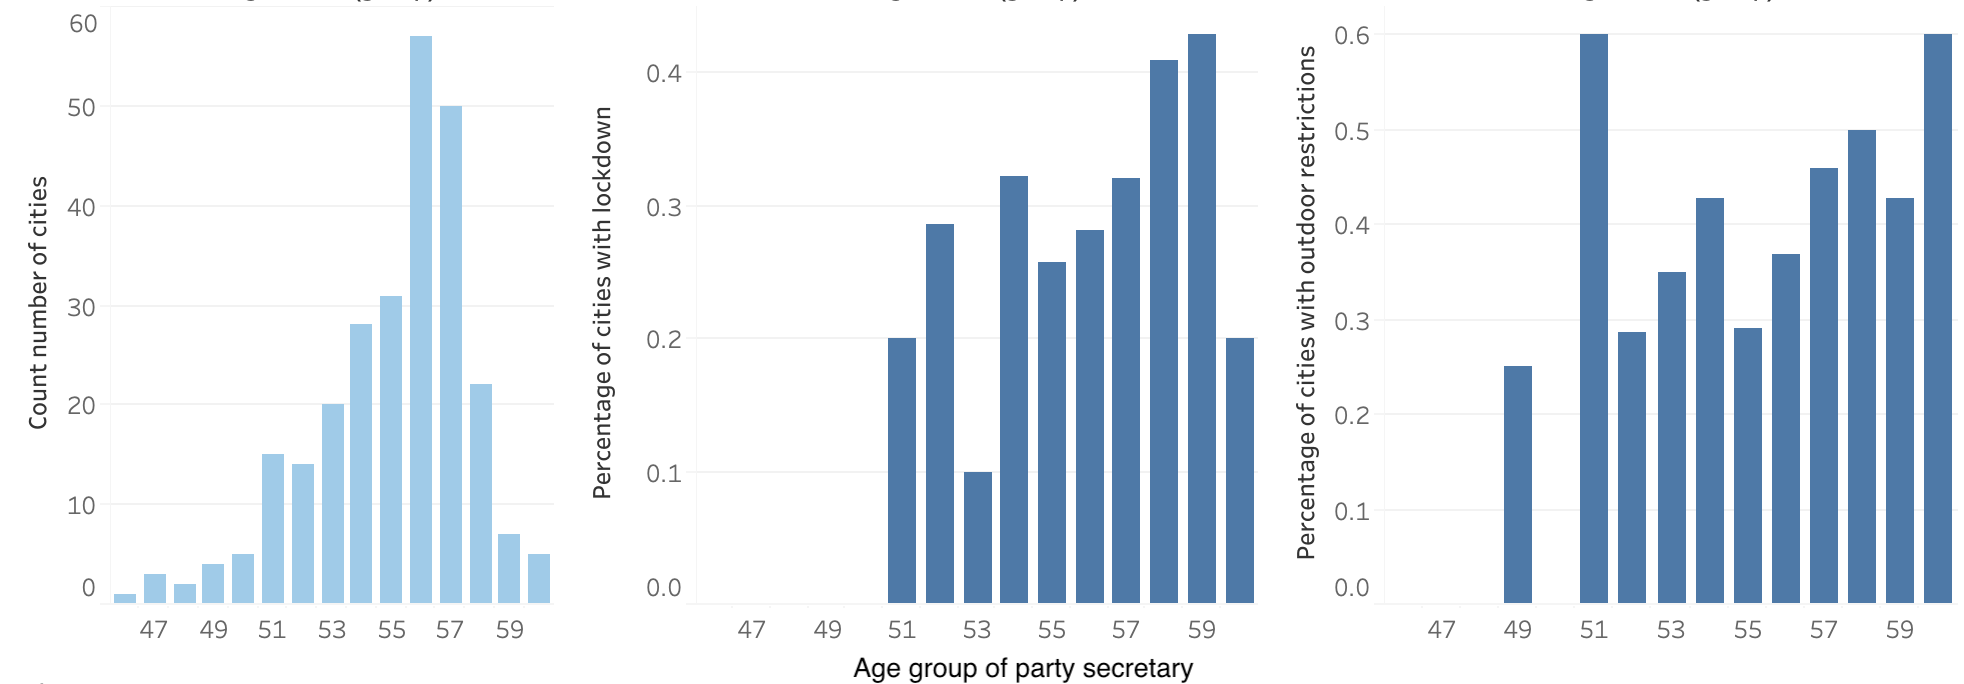
\includegraphics[width=1\textwidth]{graphs/age_group_avg} %插入图片,[]中设置图片大小,{}中是图片文件名
\caption{\%Policy implemented by secretary age group} %最终文档中希望显示的图片标题
\label{fig.1} %用于文内引用的标签
\end{figure}


\section{Empirical Results} 

In the following studies, I remove the 12 cities in Hubei, because Hubei, as the province where the virus was first identified, had disproportionately more confirmed COVID cases and officials have adopted the most strict policies. I conjecture that the motivation and behavior of Hubei officials are likely to be different than most other regions. The four direct-controlled municipalities (Beijing, Shanghai, Tianjin, and Chongqin) are also ignored, because their administrative ranking is comparable to provinces, and should be not compared with the city-level governments.

\subsection{Regression with control variables}

To depict the relationship between secretary age and the likelihood of, I used the the policy dummy (1 for policy adopted, 0 for not) as the dependent variable, and use multinomial logistic regression to fit the model. 

The independent variable, secretary age, refers to the city party secretry's age in February 2020, rounded to the closest integer. Besides age, I conjecture that the most important factor that local leaders consider when making policies is the total number of confirmed cases. Since the policy dummy records whether the city adopted the policy by the end of February, the control variable COVID case records the number of confirmed cases on Feb 25, 2020 in that city.

I also incorporate two groups of controls. Province dummies is a 25-dimension dummy that indicates which of the 25 provinces the particular city is in. City characteristics refers to 5 covariates that I believe are important to the transmission and containment of the pandemic: 1) log population in 2018, 2) GDP per 10,000 population, 3) population density, 4) percentage of employment in the secondary industry 5) number of doctors per 10,000 population. These variables can accurately depict city size, level of development, potential speech of virus transmission, industrial structure, and level of medicare, and should cover most factors party secretary consider when making decisions.



\begin{table}[H]
\caption{logistic regression on two policy measures}
\begin{center}
\begin{tabular}{l c c c c c c c c}
\hline
dependent: & \multicolumn{4}{l}{lockdown}  & \multicolumn{4}{l}{outdoor restriction}\\
\hline
secretary age  & $0.17^{***}$ & $0.16^{**}$  & $0.18^{*}$   & $0.15^{**}$ & $0.11^{**}$ & $0.10^{*}$  & $0.09$    & $0.09^{*}$   \\
               & $(0.06)$     & $(0.06)$     & $(0.10)$     & $(0.07)$    & $(0.05)$    & $(0.05)$    & $(0.06)$  & $(0.05)$     \\
COVID case     &              & $0.01^{***}$ & $0.04^{***}$ & $0.01^{**}$ &             & $0.01^{**}$ & $0.00$    & $0.01^{***}$ \\
               &              & $(0.00)$     & $(0.01)$     & $(0.00)$    &             & $(0.00)$    & $(0.00)$  & $(0.00)$     \\
province dummies &-&-&Yes&-&-&-&Yes&- \\
(n=25)\\
city characteristics &-&-&-&Yes&-&-&-&Yes \\
(n=5)\\

\hline
Num. obs.      & $264$        & $264$        & $264$        & $264$        & $264$        & $264$        & $264$       & $264$        \\
\hline
\multicolumn{9}{l}{\scriptsize{$^{***}p<0.01$; $^{**}p<0.05$; $^{*}p<0.1$}}
\end{tabular}
\label{Table 1}
\end{center}
\end{table}


In general, there is a clear positive relationship between secretary age and likelihood of lockdown, meaning that an older secretary is likely to be risk-averse. The relation is stronger for the lockdown, but is also present in the outdoor restriction measure.  Possibly due to the large number of independent variables compared to dependent variables, the regression involving province dummies have lower significance level.

To further test for the robustness of the above results, I use an alternative measure of age. Work age refers to the duration that the city secretary has joined the labor market. Even if her first job is not in the government, it is still counted as work age. This is another common measure used in Chinese government reports to rule out the effect of factors like different education levels. 

\begin{table}[H]
\caption{alternative measure of age}
\begin{center}
\begin{tabular}{l c c c c c c c c}
\hline
dependent: & \multicolumn{4}{l}{lockdown}  & \multicolumn{4}{l}{outdoor restriction}\\
\hline
work\_age      & $0.11^{***}$ & $0.12^{***}$ & $0.13^{*}$   & $0.11^{**}$ & $0.10^{***}$ & $0.10^{***}$ & $0.08^{**}$ & $0.11^{***}$ \\
               & $(0.04)$     & $(0.04)$     & $(0.07)$     & $(0.04)$    & $(0.03)$     & $(0.04)$     & $(0.04)$    & $(0.04)$     \\

COVID case     &              & $0.01^{***}$ & $0.04^{***}$ & $0.01^{**}$ &              & $0.01^{**}$  & $0.00$      & $0.01^{***}$ \\
               &              & $(0.00)$     & $(0.01)$     & $(0.00)$    &              & $(0.00)$     & $(0.00)$    & $(0.00)$     \\
province dummies &-&-&Yes&-&-&-&Yes&- \\
(n=25)\\
city characteristics &-&-&-&Yes&-&-&-&Yes \\
(n=5)\\

\hline
Num. obs.      & $264$        & $264$        & $264$        & $264$        & $264$        & $264$        & $264$       & $264$        \\
\hline
\multicolumn{9}{l}{\scriptsize{$^{***}p<0.01$; $^{**}p<0.05$; $^{*}p<0.1$}}
\end{tabular}
\label{Table 1}
\end{center}
\end{table}

Observe that the results are much stronger significance for all policy measures and control variables. Since work age is a better measure of working experience than age, this increased significance corresponds to the theory of Prendergast and Stole that past working experience is the source of risk-averse behaviors.

The results above are also repeated for linear regression, and similar patterns are observed. Regression tables are attached in appendix. 

%\subsection{Survival analysis}


%\subsection{RD Design}
%
%There are evidence showing that the effect of age on official behavior might be correlated with 

\subsection{Additional Explorations} 

\subsubsection{Mayor age effect}

As the second most powerful leader of the city, mayor might also have significant influence in policy-making. I also collected age, and work age information for city mayors in Feb 2020, and added to the baseline regressions above. Although mayor did extract some of the party secretary effects, since party secretary has the final decision on the most important issues, the influence of mayor age/work age is less than that of party secretary, measured in both magnitude and significance. Detailed regression tables are in the appendix.


\subsubsection{RD Design}

There are prior evidence showing that the effect of the age of city leader is not gradual but abrupt, and the break point is closely related to the mechanism of promotion and forced retirement. For example, Huang et al 2020 shows that the motivation for economic reform sharply changes around the age 57.5 of local city leaders. 

I used regression discontinuity to explore this effect. However, with the set of controls explored above, there is no significant break point in the range of age or work range considered. As an urgent public health crisis, local officials might not be able carefully think through the career implications, and did not fully incorporate the subtle details of their career concerns into the decision-making process. 

%\subsubsection{Real vs. Formal Policy}
%
%We should notice that the datasets above are only measures of the reported policies, but cannot reflect the actual intensity of policy implementation. To directly measure the effect of policies, I collected data from Baidu Qianxi intra-city activity index. Using big data of cellular phone, this index measures the intensity of intra-city movements. Based on that, I constructed a Policy Intensity Index (PII) at day $d$: 
%
%$$
%	\text{PII}_d = \text{Baidu index 2019}_d - \text{Baidu index 2020}_d
%$$
%
%Except for a few cities, the activity intensity in 2020 on the corresponding day is much lower. The larger the difference is, the more




\section{Conclusion}

In this paper, I examines the behavior of local Chinese officials during the COVID-19 pandemic from a principal-agent perspective. I discovered that age influences the risk-preference behaviors of party secretaries, and older officials are more likely to implement stringent policies to minimize risk. In addition, the effect is stronger if measured in work age, and this fact confirms to the Prendergast and Stole's model that the more working experience the manager has, the more risk-averse she will be. 



\begin{thebibliography}{999}	

% covid fact and research 
\bibitem{inner mongolia}
	Inner Mongolia http://wjw.nmg.gov.cn/doc/2020/02/14/292018.shtml

%\bibitem{xjp urges}
%	Xinhua net, http://www.xinhuanet.com/politics/leaders/2020-01/20/c_1125486561.htm

\bibitem{chezhi}
	https://www.reuters.com/article/hubei-reshuffling-0213-thur-idCNKBS2070EW
\bibitem{yuhang}
	He, G., Pan, Y., \& Tanaka, T. (2020). The short-term impacts of COVID-19 lockdown on urban air pollution in China. Nature Sustainability, 3(12), 1005-1011.
\bibitem{bdidx}
	百度迁徙 https://qianxi.baidu.com/
\bibitem{xichen}
	Qiu, Y., Chen, X., \& Shi, W. (2020). Impacts of social and economic factors on the transmission of coronavirus disease 2019 (COVID-19) in China. Journal of Population Economics, 1.
\bibitem{57.5 age RD}
	Huang, Z., Liu, J., Ma, G., \& Xu, L. C. (2020). The Transformative Effects of Privatization in China: A Natural Experiment Based on Politician Career Concern. World Bank Policy Research Working Paper, (9261).
\bibitem{RD design}
	Lee, D. S., \& Lemieux, T. (2010). Regression discontinuity designs in economics. Journal of economic literature, 48(2), 281-355.
% 中国政府结构
\bibitem{zxg}
	周雪光. (2017). 中国国家治理的制度逻辑. 北京: 生活· 读书· 新知三联书店.
\bibitem{renqi}
	耿曙, 庞保庆, \& 钟灵娜. (2016). 中国地方领导任期与政府行为模式: 官员任期的政治经济学. 经济学 (季刊), 15(3), 893-916.
\bibitem{gdp contest}
	周黎安. (2007). 中国地方官员的晋升锦标赛模式研究 (Doctoral dissertation).
\bibitem{tuixiu}
	https://baike.baidu.com/item/%E5%85%9A%E6%94%BF%E9%A2%86%E5%AF%BC%E5%B9%B2%E9%83%A8%E9%80%80%E4%BC%91%E5%B9%B4%E9%BE%84%E8%A7%84%E5%AE%9A/16587018
\bibitem{tenure effect}
	耿曙, 庞保庆, \& 钟灵娜. (2016). 中国地方领导任期与政府行为模式: 官员任期的政治经济学. 经济学 (季刊), 15(3), 893-916.
\bibitem{mayor age effect}
	金刚, \& 沈坤荣. (2019). 地方官员晋升激励与河长制演进: 基于官员年龄的视角''. 财贸经济, 4.
\bibitem{age and tenure effect 2}
	杨刚强, 程恒祥, 吴斯 (2020), 晋升压力、官员任期与公共服务供给效率———基于中国70个城市的实证

%数据
\bibitem{wiki}
	zh.wikipedia.org
\bibitem{official info}
	http://ldzl.people.com.cn/dfzlk/front/firstPage.htm

%principal-agent
\bibitem{holmstrom and roberts 1998}
	Holmstrom, B., \& Roberts, J. (1998). The boundaries of the firm revisited. Journal of Economic perspectives, 12(4), 73-94.

\bibitem{serfling2014}
	Serfling, M. A. (2014). CEO age and the riskiness of corporate policies. Journal of Corporate Finance, 25, 251-273.
\bibitem{holmstrom1999}
  Holmström, B. (1999). Managerial incentive problems: A dynamic perspective. The review of Economic studies, 66(1), 169-182. 
\bibitem{herd behavior}
	Scharfstein, D. S., \& Stein, J. C. (1990). Herd behavior and investment. The American economic review, 465-479.
%\bibitem{hirshleifer}
%	Hirshleifer, D., \& Suh, Y. (1992). Risk, managerial effort, and project choice. Journal of Financial Intermediation, 2(3), 308-345.
\bibitem{impetuous}
	Prendergast, C., \& Stole, L. (1996). Impetuous youngsters and jaded old-timers: Acquiring a reputation for learning. Journal of political Economy, 104(6), 1105-1134.
\end{thebibliography}


%\newpage
\appendix
\section{Supplementary Regression Tables}

\subsection{Linear regression results}
\begin{table}[H]
\caption{linear regression on two policy measures}
\begin{center}
\begin{tabular}{l c c c c c c c c}
\hline
dependent: & \multicolumn{4}{l}{lockdown}  & \multicolumn{4}{l}{outdoor restriction}\\
\hline
secretary age & $0.03^{***}$ & $0.03^{**}$  & $0.01^{*}$   & $0.02^{**}$ & $0.02^{**}$ & $0.02^{*}$  & $0.02$   & $0.02^{*}$   \\
              & $(0.01)$     & $(0.01)$     & $(0.01)$     & $(0.01)$    & $(0.01)$    & $(0.01)$    & $(0.01)$ & $(0.01)$     \\
COVID case    &              & $0.00^{***}$ & $0.00^{***}$ & $0.00^{**}$ &             & $0.00^{**}$ & $0.00$   & $0.00^{***}$ \\
              &              & $(0.00)$     & $(0.00)$     & $(0.00)$    &             & $(0.00)$    & $(0.00)$ & $(0.00)$     \\
province dummies &-&-&Yes&-&-&-&Yes&- \\
(n=25)\\
city characteristics &-&-&-&Yes&-&-&-&Yes \\
(n=5)\\

\hline
R$^2$         & $0.03$       & $0.11$       & $0.59$       & $0.16$      & $0.02$      & $0.04$      & $0.28$   & $0.11$       \\
Adj. R$^2$    & $0.03$       & $0.11$       & $0.54$       & $0.13$      & $0.01$      & $0.03$      & $0.20$   & $0.08$       \\
Num. obs.     & $264$        & $264$        & $264$        & $264$       & $264$       & $264$       & $264$    & $264$        \\
\hline
\multicolumn{9}{l}{\scriptsize{$^{***}p<0.01$; $^{**}p<0.05$; $^{*}p<0.1$}}
\end{tabular}
\label{Table 1}
\end{center}
\end{table}

%%%%%%%%%%%%%%%%%%%%%%%%%%%%%%%%%%%%%%%%

\begin{table}[H]
\caption{linear regression: alternative age measure}
\begin{center}
\begin{tabular}{l c c c c c c c c}
\hline
dependent: & \multicolumn{4}{l}{lockdown}  & \multicolumn{4}{l}{outdoor restriction}\\
\hline
work\_age  & $0.02^{***}$ & $0.02^{***}$ & $0.01^{**}$  & $0.02^{***}$ & $0.02^{***}$ & $0.02^{***}$ & $0.02^{**}$ & $0.02^{***}$ \\
           & $(0.01)$     & $(0.01)$     & $(0.01)$     & $(0.01)$     & $(0.01)$     & $(0.01)$     & $(0.01)$    & $(0.01)$     \\
COVID case &              & $0.00^{***}$ & $0.00^{***}$ & $0.00^{***}$ &              & $0.00^{***}$ & $0.00$      & $0.00^{***}$ \\
           &              & $(0.00)$     & $(0.00)$     & $(0.00)$     &              & $(0.00)$     & $(0.00)$    & $(0.00)$     \\
province dummies &-&-&Yes&-&-&-&Yes&- \\
(n=25)\\
city characteristics &-&-&-&Yes&-&-&-&Yes \\
(n=5)\\

\hline
R$^2$      & $0.03$       & $0.12$       & $0.59$       & $0.16$       & $0.03$       & $0.06$       & $0.29$      & $0.13$       \\
Adj. R$^2$ & $0.03$       & $0.12$       & $0.54$       & $0.14$       & $0.03$       & $0.05$       & $0.21$      & $0.10$       \\
Num. obs.  & $264$        & $264$        & $264$        & $264$        & $264$        & $264$        & $264$       & $264$        \\
\hline
\multicolumn{9}{l}{\scriptsize{$^{***}p<0.01$; $^{**}p<0.05$; $^{*}p<0.1$}}
\end{tabular}
\label{Table 1}
\end{center}
\end{table}

%%%%%%%%%%%%%%%%%%%%%%%%%%%%%%%%%%%%%%%%
\subsection{Mayor added as control}
% 下面是考虑mayor age 
\begin{table}[H]
\caption{logistic regression for age (mayor added as control)}
\begin{center}
\begin{tabular}{l c c c c c c c c}
\hline
 & 1a & 1b & 1c & 1d & 2a & 2b & 2c & 2d \\
\hline
secretary age  & $0.16^{***}$ & $0.15^{**}$  & $0.17^{*}$   & $0.15^{**}$ & $0.09^{*}$ & $0.09^{*}$  & $0.08$    & $0.08$       \\
               & $(0.06)$     & $(0.06)$     & $(0.10)$     & $(0.07)$    & $(0.05)$   & $(0.05)$    & $(0.06)$  & $(0.05)$     \\
mayor\_age     & $0.03$       & $0.01$       & $0.03$       & $-0.00$     & $0.07^{*}$ & $0.06^{*}$  & $0.07$    & $0.09^{**}$  \\
               & $(0.04)$     & $(0.04)$     & $(0.06)$     & $(0.04)$    & $(0.04)$   & $(0.04)$    & $(0.05)$  & $(0.04)$     \\
COVID case     &              & $0.01^{***}$ & $0.04^{***}$ & $0.01^{**}$ &            & $0.01^{**}$ & $0.00$    & $0.01^{***}$ \\
               &              & $(0.00)$     & $(0.01)$     & $(0.00)$    &            & $(0.00)$    & $(0.00)$  & $(0.00)$     \\
province dummies &-&-&Yes&-&-&-&Yes&- \\
(n=25)\\
city characteristics &-&-&-&Yes&-&-&-&Yes \\
(n=5)\\

\hline
Num. obs.      & $264$        & $264$        & $264$        & $264$       & $264$      & $264$       & $264$     & $264$        \\
\hline
\multicolumn{9}{l}{\scriptsize{$^{***}p<0.01$; $^{**}p<0.05$; $^{*}p<0.1$}}
\end{tabular}
\label{Table 1}
\end{center}
\end{table}
%%%%%%%%%%%%%%%%%%%%%%%%%%%%%%%%%%%%%%%%
\begin{table}[H]
\caption{logistic regression for work age with (mayor added as control)}
\begin{center}
\begin{tabular}{l c c c c c c c c}
\hline
 & 1a & 1b & 1c & 1d & 2a & 2b & 2c & 2d \\
\hline
work\_age        & $0.11^{***}$ & $0.12^{***}$ & $0.12^{*}$   & $0.11^{**}$ & $0.10^{***}$ & $0.10^{***}$ & $0.08^{**}$ & $0.11^{***}$ \\
                 & $(0.04)$     & $(0.04)$     & $(0.07)$     & $(0.04)$    & $(0.04)$     & $(0.04)$     & $(0.04)$    & $(0.04)$     \\
mayor\_work\_age & $0.04$       & $0.03$       & $0.08$       & $0.02$      & $0.06^{**}$  & $0.05^{*}$   & $0.07^{*}$  & $0.06^{**}$  \\
                 & $(0.03)$     & $(0.03)$     & $(0.06)$     & $(0.03)$    & $(0.03)$     & $(0.03)$     & $(0.04)$    & $(0.03)$     \\
COVID case       &              & $0.01^{***}$ & $0.03^{***}$ & $0.01^{**}$ &              & $0.01^{**}$  & $0.00$      & $0.01^{***}$ \\
                 &              & $(0.00)$     & $(0.01)$     & $(0.00)$    &              & $(0.00)$     & $(0.00)$    & $(0.00)$     \\
province dummies &-&-&Yes&-&-&-&Yes&- \\
(n=25)\\
city characteristics &-&-&-&Yes&-&-&-&Yes \\
(n=5)\\
\hline
Num. obs.        & $264$        & $264$        & $264$        & $264$       & $264$        & $264$        & $264$       & $264$        \\
\hline
\multicolumn{9}{l}{\scriptsize{$^{***}p<0.01$; $^{**}p<0.05$; $^{*}p<0.1$}}
\end{tabular}
\label{Table 1}
\end{center}
\end{table}









\end{CJK}
\end{document}